We describe in this section a simulation-based method that provides an alternative estimate of the data-driven backgrounds described in Sections ~\ref{sec:chargeflip} and ~\ref{subsec:fakes_matrix}. 
 %More details about the method can be found in Appendix \ref{app_mc_template}.

The MC-based method relies on kinematic distributions from MC simulations to extrapolate background predictions from 
control regions with low \met , \meff , 
and jet multiplicity to the signal regions (where \met , \meff , or jet multiplicity are required to be high). 
The control regions are used to reweight MC simulation of \ttbar\ and $V+$ jets events to match the observed data 
by extracting correction factors which depend on the identified origin of the fake or non-prompt lepton. 
The main assumption of the method is that the MC simulations describe the kinematic distributions correctly 
and predict accurately the rate of fake leptons up to a global factor (for each type of fake lepton) 
independent of the event kinematics and the process type. This assumption makes the method a suitable cross-check of the matrix method, 
that assumes that the lepton fake rates are the same in control and signal regions regardless of the selection requirements. 
The other assumption the MC template method makes is that the fake rates are uncorrelated in events with multiple fake leptons 
which is expected to be negligeable.

Six non-overlapping control regions are defined by the presence of $b$-jets and by the flavors of the same sign lepton pair in the event:
\begin{itemize}
\item CR0b: events without $b$-jets in $ee$, $e\mu$, and $\mu\mu$ channels.
\item CR1b: events with at least one $b$-jet in $ee$, $e\mu$, and $\mu\mu$ channels.
\end{itemize}
All the selected events contain two or more same-sign signal leptons and \met >40 GeV and 2 or more jets. 
Events satisfying the signal regions requirements are excluded from the control regions. 
The purpose of the \met requirement is to remove multi-jet events that have two or more ``fake'' leptons and tend to have low \met. 

The next step is to classify events into separate categories depending on the lepton origin. 
The three main categories are prompt isolated leptons, charge flipped electrons, 
and ``fake'' leptons which consist of non-prompt leptons coming from hadron decays and hadrons misidentified as leptons. 
The fakes are further separated by the lepton flavor ($e$ or $\mu$) and by the jet flavor producing the fake lepton. 
We separate the leptons that are coming from $b$-hadron decays, 
labelled as heavy-flavor (HF), from the rest of the fakes, labelled as light-flavor (LF), and derive a fake rate correction for 
each category. The purpose of this separation is to make the $b$-tagging requirement orthogonal to the fake rate correction. 
The classification is done based on the parent particle from the generator event record using the type and origin of the lepton provided 
by the MCTruthClassifier.

In total we have five categories (charge flip, EL HF, MU HF, EL LF, MU LF) that we derive correction factors for using a simulatenous fit to data in six control regions (CR0b and CR1b for $ee$, $e\mu$, and $\mu\mu$ channels).
The fit uses a likelihood function defined as the product of the Poisson probabilities describing the observed events in the binned 
distributions from the expected number 
of events rescaled by the five correction factors which are left free to float in the fit.  
These correction factors are applied to the MC predictions in the signal regions to obtain an estimation of the fake and charge flip backgrounds. 

The six distributions are chosen for variables that provide the best separation between processes with prompt leptons and processes with fake leptons and charge flip and are shown 
before and after the fit in Figures \ref{f:prefit_CR0b}-\ref{f:prefit_CR1b} and Figures \ref{f:postfit_CR0b}-\ref{f:postfit_CR1b}, respectively. 

 \begin{figure}[htb]
   \includegraphics[width=.32\textwidth]{Prefit/el2_pt_ee_CR0b_SS3L}
   \includegraphics[width=.32\textwidth]{Prefit/NJETS_em_CR0b_SS3L}
   \includegraphics[width=.32\textwidth]{Prefit/mu2_pt_mm_CR0b_SS3L}
 \caption{
 Pre-fit distributions for  $ee$ channel (left),  for  $e\mu$ channel (middle), and  for  $\mu\mu$ channel (right) from CR0b that were used in the fit to extract the fake rate and charge flip corrections.
The generator used in these plots is Powheg. The hashed band represents the sum of systematic uncertainties on the predictions.
 \label{f:prefit_CR0b}
 }
 \end{figure}

\begin{figure}[htb]
  \includegraphics[width=.32\textwidth]{Postfit/el2_pt_ee_CR0b_SS3L}
  \includegraphics[width=.32\textwidth]{Postfit/NJETS_em_CR0b_SS3L}
  \includegraphics[width=.32\textwidth]{Postfit/mu2_pt_mm_CR0b_SS3L}
\caption{
Post-fit distributions for  $ee$ channel (left),  for  $e\mu$ channel (middle), and  for  $\mu\mu$ channel (right) from CR0b that were used in the fit to extract the fake rate and charge flip corrections.
The generator used in these plots is Powheg. The hashed band represents the sum of systematic uncertainties on the predictions.
\label{f:postfit_CR0b}
}
\end{figure}

 \begin{figure}[htb]
   \includegraphics[width=.32\textwidth]{Prefit/el2_pt_ee_CR1b_SS3L}
   \includegraphics[width=.32\textwidth]{Prefit/NJETS_em_CR1b_SS3L}
   \includegraphics[width=.32\textwidth]{Prefit/mu2_pt_mm_CR1b_SS3L}
 \caption{
 Pre-fit distributions for  $ee$ channel (left), for  $e\mu$ channel (middle), and  for  $\mu\mu$ channel (right) from CR1b that were used in the fit to extract the fake rate and charge flip corrections.
The generator used in these plots is Powheg. The hashed band represents the sum of systematic uncertainties on the predictions.
 \label{f:prefit_CR1b}
 }
 \end{figure}

\begin{figure}[htb]
  \includegraphics[width=.32\textwidth]{Postfit/el2_pt_ee_CR1b_SS3L}
  \includegraphics[width=.32\textwidth]{Postfit/NJETS_em_CR1b_SS3L}
  \includegraphics[width=.32\textwidth]{Postfit/mu2_pt_mm_CR1b_SS3L}
\caption{
Post-fit distributions for  $ee$ channel (left), for  $e\mu$ channel (middle), and  for  $\mu\mu$ channel (right) from CR1b that were used in the fit to extract the fake rate and charge flip corrections.
The generator used in these plots is Powheg. The hashed band represents the sum of systematic uncertainties on the predictions.
\label{f:postfit_CR1b}
}
\end{figure}

The minimization of the negative log likelihood using the \textsc{Minuit} package leads 
to the correction factor shown in Tables \ref{t:fake_factors_powheg} and \ref{t:fake_factors_sherpa}.
The tables represent the correction factors obtained from the fit upon using two different parton showers, Pythia and Sherpa
for the processes that lead to non-prompt leptons and charge flips.
The goal of varying the parton shower is to access the dependence of the fake and charge flip estimates on the choice of the 
parton shower. An additional systematic uncertainty is added to account for this dependency. 
The uncertainties in the correction factors themselves correspond to how much the parameter needs to be varied for 
a one standard deviation change in the likelihood function. This uncertainty takes into account the limited number of simulated events and is included as a 
systematic uncertainty on the expected number of background events. 


\begin{table}[htb]
  \caption{The fake-rate and charge flip corrections obtained after minimizing the likelihood function using Pythia.
    The uncertainty in the corrections takes into account the limited statistics of simulated events.
    \label{t:fake_factors_powheg}}
  \centering
  % % \scalebox{0.85}{
   \begin{tabular}{|c|c|c|}
          \hline
          Category & Correction & Uncertainty  \\
          \hline
          chFlip & 1.49 & 0.58 \\ 
          HF EL & 2.80 & 0.98 \\
          LF EL & 2.89 & 0.88 \\
          HF MU & 1.59 & 0.31 \\
          LF MU & 1.00 & 1.34 \\
          \hline
        \end{tabular}
  % % }                                                                            
\end{table}

\begin{table}[htb]
  \caption{The fake-rate and charge flip corrections obtained after minimizing the likelihood function using Sherpa.
    The uncertainty in the corrections takes into account the limited statistics of simulated events.
    \label{t:fake_factors_sherpa}}
  \centering
  % % \scalebox{0.85}{
  \begin{tabular}{|c|c|c|}
    \hline
    Category & Correction & Uncertainty  \\
    \hline
    chFlip & 1.34 & 0.58 \\ 
    HF EL & 2.40 & 0.85 \\
    LF EL & 1.83 & 1.04 \\
    HF MU & 1.17 & 0.16 \\
    LF MU & 2.40 & 0.81 \\
    \hline
  \end{tabular}                                                                                         
  % % }                                                                            
\end{table}


The MC template method is validated by looking at the Data/MC agreement near the signal regions where we invert one of the cuts while keeping the last bin corresponding to the SR blinded. These distributions can be found in Appendix~\ref{app:mctemplate}.

After applying the correction factors of Table \ref{t:fake_factors_powheg} to obtain the nominal fake estimates with the samples shown 
in Table \ref{t:samples_pythia}, 
an additional uncertainty on the rate of fake leptons from \ttbar and $V$+jets in the signal region is assigned by repeating the background evaluation 
procedure using samples with Sherpa shown in Tables~\ref{t:samples_sherpa1}-\ref{t:samples_sherpa2} and with the correction factors from 
Table \ref{t:fake_factors_sherpa}. 
In practice, only \ttbar contributes to the SRs and the final yields with systamtic uncertainties from 
fit uncertainty, theory uncertainties on ttbar, comparison of different showers (Pythia 6 and Sherpa) is shown in Table \ref{tab:fakes_mcglobal}.
This table also shows a global correction factor derived by taking the ratio of the weighted \ttbar to raw MC \ttbar with
a global uncertainty that includes all systematic uncertainties used to obtain the final estimate. 


\begin{table}[!htb]
\caption{Expected yields for background processes with fake leptons,
in the signal regions with a global correction factor that represents the ratio of weighted \ttbar to raw MC \ttbar with
a global uncertainty that includes: fit uncertainty, theory uncertainties on ttbar, comparison of different showers. 
The fraction of the systematic uncertainty from the comparison between two showers (Pythia and Sherpa) is also shown.
}
\label{tab:fakes_mcglobal}
\centering
\resizebox{\textwidth}{!}{
\begin{tabular}{|c||c|c|c||}\hline
Region &              MC Template method  & Global correction & Shower systematic \\
\hline
Rpc2L0bH & $1.00 \pm 0.96 \pm 0.81$ & $2.80 \pm 2.10$ & 74\% \\
Rpc2L0bS & $1.68 \pm 1.02 \pm 1.26$ & $2.89 \pm 1.97$ & 65\% \\
Rpc2L1bH & $2.07 \pm 0.63 \pm 1.56$ & $1.22 \pm 1.14$ & 34\% \\
Rpc2L1bS & $2.33 \pm 1.17 \pm 2.10$ & $1.83 \pm 1.42$ & 81\% \\
Rpc2L2bH & $<0.5$ & $0 \pm 0$ & 0\% \\
Rpc2L2bS & $0.41 \pm 0.33 \pm 0.45$ & $1.47 \pm 1.12$ & 73\% \\
Rpc2Lsoft1b & $2.48 \pm 1.32 \pm 1.86$ & $1.59 \pm 1.31$ & 68\% \\
Rpc2Lsoft2b & $1.66 \pm 0.66 \pm 1.28$ & $1.72 \pm 1.29$ & 54\% \\
Rpc3L0bH & $<0.5$ & $0 \pm 0$ & 0\% \\
Rpc3L0bS & $0.21 \pm 0.15 \pm 0.16$ & $2.90 \pm 2.20$ & 71\% \\
Rpc3L1bH & $0.42 \pm 0.29 \pm 0.32$ & $1.59 \pm 1.25$ & 59\% \\
Rpc3L1bS & $3.55 \pm 1.80 \pm 2.76$ & $1.76 \pm 1.32$ & 67\% \\
Rpc3LSS1b & $0.90 \pm 0.14 \pm 0.69$ & $2.34 \pm 1.44$ & 56\% \\
Rpv2L0b & $1.02 \pm 0.96 \pm 0.76$  & $2.80 \pm 2.10$ & 66\% \\
Rpv2L1bH & $0.60 \pm 0.35 \pm 0.48$ & $1.32 \pm 0.92$ & 45\% \\
Rpv2L1bM & $1.20 \pm 0.69 \pm 0.95$ & $1.59 \pm 1.25$ & 58\% \\
Rpv2L1bS & $4.46 \pm 1.67 \pm 3.45$ & $1.33 \pm 0.80$ & 67\% \\
Rpv2L2bH & $<0.5$ & $0 \pm 0$ & 0\% \\
Rpv2L2bS & $7.24 \pm 2.36 \pm 5.43$ & $2.45 \pm 1.83$ & 73\% \\
\hline
\hline
\end{tabular}
}
\end{table}
